\subsection{The Geometric Effective Action and Lagrangians of Cosmochrony $\left(\mathcal{L}_{\mathrm{CC}}\right)$}
  \label{subsec:the-geometric-effective-action-and-lagrangians-of-cosmochrony-Lcc}

  \subsubsection*{Interpretational caution.}
    The action principle presented below employs conventional field-theoretic notation, including a metric tensor
    $g_{\mu \nu}$ and a four-dimensional integration measure.
    This should not be interpreted as assuming pre-existing spacetime structure.

    The formalism serves two purposes:
    \begin{enumerate}
      \item To provide a compact representation of $\chi$ dynamics in regimes where an effective spacetime description is valid.
      \item To establish the bridge between the fundamental relational network and the effective manifold description used in standard physics.
    \end{enumerate}

    The fundamental content of the theory is the field $\chi$ and its relaxation dynamics on a discrete graph.
    The metric $g_{\mu \nu}$ appearing in the action is a statistical emergent structure representing the connectivity
    and correlation density of the $\chi$ field, not an independent ontological input.

  \subsubsection*{Discrete Network Foundation}
    The dynamics of $\chi$ are fundamentally defined on a \textbf{discrete network}, where each node $i$ represents a
    local value $\chi_i$, and each link between nodes $i$ and $j$ is characterized by a \textbf{connectivity strength}
    $K_{ij}$.
    This matrix $K_{ij}$ encodes the correlation between neighboring $\chi$-values and serves as the microscopic
    foundation for the emergent geometry.
    In regimes where $\chi$ admits a quasi-stable geometric interpretation, $K_{ij}$ can be mapped to an effective
    metric $g_{\mu\nu}$ through the relation:
    \[
      g_{\mu\nu} dx^\mu dx^\nu \approx \sum_{(u,v) \in \text{path}} \frac{1}{K_{uv}}
    \]
    Here, $K_{ij}$ is not a static background but a dynamic measure of the local $\chi$-field gradient, representing the
    \textbf{relational tension} between nodes.
    This definition ensures that the geometry is a secondary consequence of the field's local state, avoiding any
    circular dependency on a pre-existing metric.

    \begin{figure}[h]
      \centering
      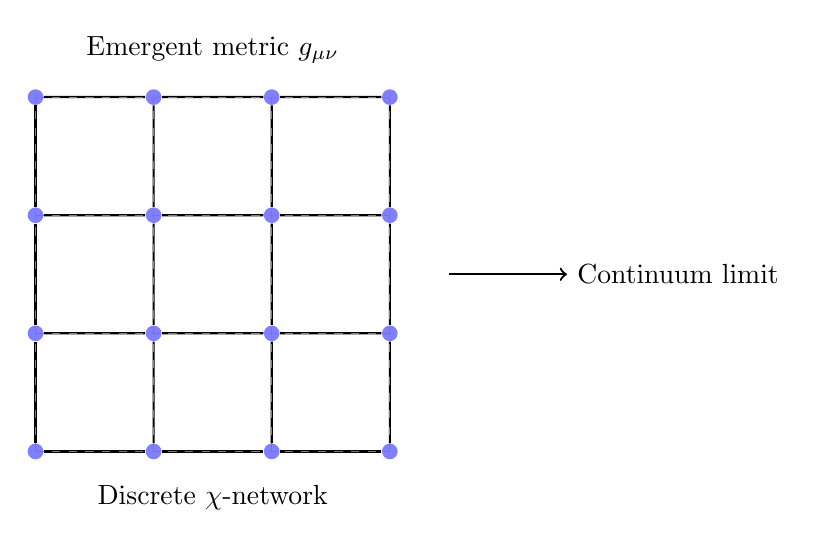
\begin{tikzpicture}[scale=1.5]
        % Nodes (chi_i values)
        \foreach \x in {0,1,2,3} {
          \foreach \y in {0,1,2,3} {
            \node[circle, fill=blue!50, inner sep=2pt] (n-\x-\y) at (\x,\y) {};
          }
        }

        % Links (K_ij)
        \foreach \x in {0,1,2} {
          \foreach \y in {0,1,2,3} {
            \draw[thick] (n-\x-\y) -- (n-\the\numexpr\x+1\relax-\y);
          }
        }
        \foreach \x in {0,1,2,3} {
          \foreach \y in {0,1,2} {
            \draw[thick] (n-\x-\y) -- (n-\x-\the\numexpr\y+1\relax);
          }
        }

        % Emergent metric (deformed grid)
        \draw[gray, dashed, thin] (0,0) grid (3,3);

        % Labels
        \node[below] at (1.5,-0.2) {Discrete $\chi$-network};
        \node[above] at (1.5,3.2) {Emergent metric $g_{\mu\nu}$};
        \draw[->, thick] (3.5,1.5) -- (4.5,1.5) node[right] {Continuum limit};
      \end{tikzpicture}
      \caption{Discrete network of $\chi$-nodes (blue dots) connected by links with strength $K_{ij}$ (line thickness).
      The emergent metric $g_{\mu\nu}$ (deformed grid) arises from the statistical properties of the network's
      connectivity, encoding spatial and temporal relations without a pre-existing background.}
      \label{fig:chi-network}
    \end{figure}

  \subsubsection*{Effective action formulation.}
    In regimes where $\chi$ admits a quasi-stable geometric interpretation, the dynamics may be encoded in an effective
    action:
    \[
      S_{\mathrm{CC}} = \int \mathcal{L}_{\mathrm{CC}} \sqrt{-g} \, d^4 x
    \]
    where the Lagrangian density decomposes as:
    \[
      \mathcal{L}_{\mathrm{CC}} = \mathcal{L}_{\text{Gravity/Time}} + \mathcal{L}_{\chi / \text{Soliton}} + \mathcal{L}_{\text{Forces/Matter}}
    \]
    The symbol $\sqrt{-g}$ represents the invariant volume element.
    In regimes where no spacetime interpretation yet exists (e.g., at the nodes of the fundamental graph), this should
    be understood as an abstract integration measure $d\mu$ on the configuration space of $\chi$.

  \subsubsection*{Status of $g_{\mu\nu}$ in this formulation.}
    The metric $g_{\mu\nu}$ is an effective description of the coupling strengths $K_{ij}$ between $\chi$ nodes.
    It is defined by the requirement that the distance $ds^2$ in the continuum matches the operational distance derived
    from the network's connectivity:
    \[
      g_{\mu\nu} dx^\mu dx^\nu \approx \sum_{(u,v) \in \text{path}} \frac{1}{K_{uv}}
    \]
    Consequently, $g_{\mu\nu}$ is a phenomenological summary of the underlying relational dynamics, capturing the local
    rate of $\chi$-relaxation and its spatial correlations.
